%% IGNORE THESE RQs

\subsection{RQ4: Does predictability depend on the design choice?}
\label{subsec:rq4}

\textbf{Finding.} Predictability varies with the intervention. Sampling temperature and second-language choice change reference BPB by 3.4 to 4.9 pooled baseline seed standard deviations and yield high agreement at 350M. The depth and language-list effects are smaller, at 1.5 to 1.6. Benchmark effects lie between 1.1 and 1.8 and show weak aggregate agreement across interventions.

\textbf{Setup.} We compare intervention effects with the variability observed across repeated baseline runs. For each intervention and language setting we measure the absolute difference between the two levels at the reference, per item, in units of that item's seed standard deviation, taken as the median over the seed-replicated cells of the baseline (deep, scheme A) at the same task. A ratio near 1 means the observed difference is comparable to this baseline variability. The denominator pools seed-replicated cells; it is neither the standard error of the intervention contrast nor a direct estimate of variability at every reference size. We then read the decision accuracy of each proxy size at its final checkpoint, as in \S\ref{subsec:rq2}, for five pairwise comparisons from the four intervention types: depth, language lists, sampling temperature ($T = 1$ against $T = 3$ at $L = 50$), and the second language at $L = 2$ (Russian against Chinese, and against Spanish). The second-language decision has one shared trained language, English, so we instead evaluate its BPB decision on languages trained by neither level.
% REVIEW: Original count: 98. Verify against the exact set difference: excluding
% English and both alternative second languages from 100 would leave 97.

\begin{figure}[t]
\centering
% figure copied from the analysis by documents/paper/figures/make_rq_figures.py -- never edit it here
% generator: https://github.com/mariagrandury/snr-multilingual/blob/feat/snr-update/src/signal-and-noise/analysis/rq05_design_decisions/analyze.py
% figure:    https://github.com/mariagrandury/snr-multilingual/blob/feat/snr-update/src/signal-and-noise/analysis/rq05_design_decisions/pretraining/predictivity_all/rq4_interventions.png
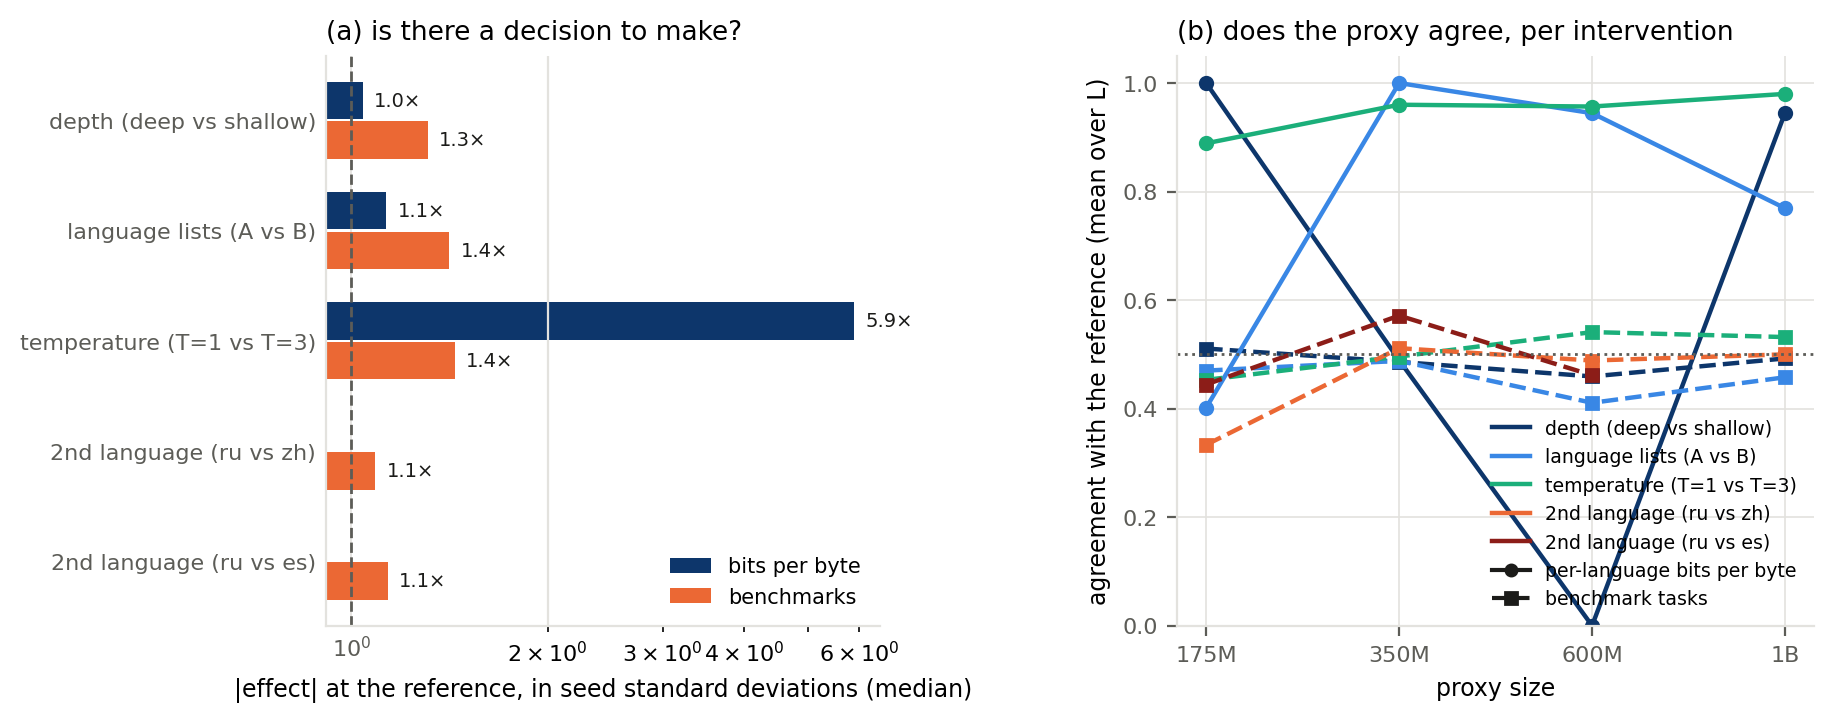
\includegraphics[width=\textwidth]{figures/rq4.png}
\caption{Does predictivity depend on the design choice. (a) Median absolute effect of each intervention at the reference, in seed standard deviations, on per-language bits per byte and on benchmark tasks; the dashed line marks a ratio of one to the pooled baseline seed standard deviation, not a significance threshold. (b) Agreement of each proxy size with the reference's final decision, averaged over language settings, on bits per byte (solid) and on benchmarks (dashed). For the second-language comparisons, BPB agreement uses languages trained by neither level. Reference sizes and evaluated populations can differ between BPB and benchmarks.}
\label{fig:rq4}
\end{figure}

\textbf{Results.} Figure~\ref{fig:rq4}a compares intervention effects relative to baseline variability. On bits per byte, the median effect at the reference is 4.9 seed standard deviations for Russian against Chinese, 3.9 for sampling temperature and 3.4 for Russian against Spanish, against 1.6 for the language lists and 1.5 for depth. On benchmarks every intervention sits between 1.1 and 1.8. Figure~\ref{fig:rq4}b shows that the proxy's reliability follows the same order. The temperature decision is read correctly on 88\% of the trained languages by 175M and 96\% by 350M, against a 600M reference; the second-language decisions on 75 to 78\% at 175M and 86 to 90\% at 350M over the never-trained languages. For language selection, 350M matches the observed reference ranking (\S\ref{subsec:rq2}); the depth comparison shows no similarly consistent transfer. On aggregate training loss, the two architectures differ by about one seed standard deviation. This small separation makes training variability a plausible contributor to the architecture result, but does not establish the cause of the 175M rank reversal.

\textbf{Benchmark comparisons.} Agreement remains weak across interventions: between 0.30 and 0.54 at every proxy size for every decision, with no gain from a larger proxy. We therefore find no consistently reliable benchmark-based decision among these comparisons. We hypothesize that the larger effects relative to variability in BPB help explain its stronger agreement. Its dense token-level observations may contribute, but byte normalization alone does not guarantee low variance, and tokens within a document are not independent.
% REVIEW: The original contrast used a 500-item accuracy; evaluate uncertainty
% with paired document/item resampling rather than equating sample counts.

\subsection{RQ5: Can scaling estimates transfer across languages?}
\label{subsec:rq5}

\textbf{Finding.} Borrowing a scaling exponent from other languages supports prediction from a single 175M measurement of the target language. Median absolute relative error at the available reference is 3.4\% for trained languages and 6.7\% for languages absent from training. The language-list decision also transfers to languages absent from training, with 76\% agreement at 600M against 94\% on shared training languages. This tests transfer with limited target-language evaluation, rather than prediction without measuring that language.

\textbf{Setup.} Bits per byte is scored on all 100 validation languages for every cell, including 45 languages absent from all training mixtures represented in this analysis. A language can also be absent at one $L$ and present at another, so we classify training exposure separately for each (language, $L$) chain. On the deep, scheme-A ladder at each $L$ we fit, per language, $\log \mathrm{BPB} = a_\ell - \alpha_\ell \log N$ on the proxy rungs. We then hold each language out in turn and predict its reference bits per byte with the median exponent of the other 99 languages at that $L$ and an intercept fitted on its own $k$ smallest rungs, for $k$ from one (175M alone) to four. We compare the relative error at the reference against the language's own fit (which needs three rungs) and against taking the largest proxy's value as the prediction. The reference is 1.7B at $L \in \{1, 2, 8, 30\}$ and 1B at $L \in \{15, 50\}$; 106 (language, $L$) chains are trained languages and 494 are not. For decisions, we read the language-list decision of \S\ref{subsec:rq2} on the languages neither scheme trains.

\begin{figure}[t]
\centering
% figure copied from the analysis by documents/paper/figures/make_rq_figures.py -- never edit it here
% generator: https://github.com/mariagrandury/snr-multilingual/blob/feat/snr-update/src/signal-and-noise/analysis/rq06_language_transfer/analyze.py
% figure:    https://github.com/mariagrandury/snr-multilingual/blob/feat/snr-update/src/signal-and-noise/analysis/rq06_language_transfer/pretraining/predictivity_all/rq5_transfer.png
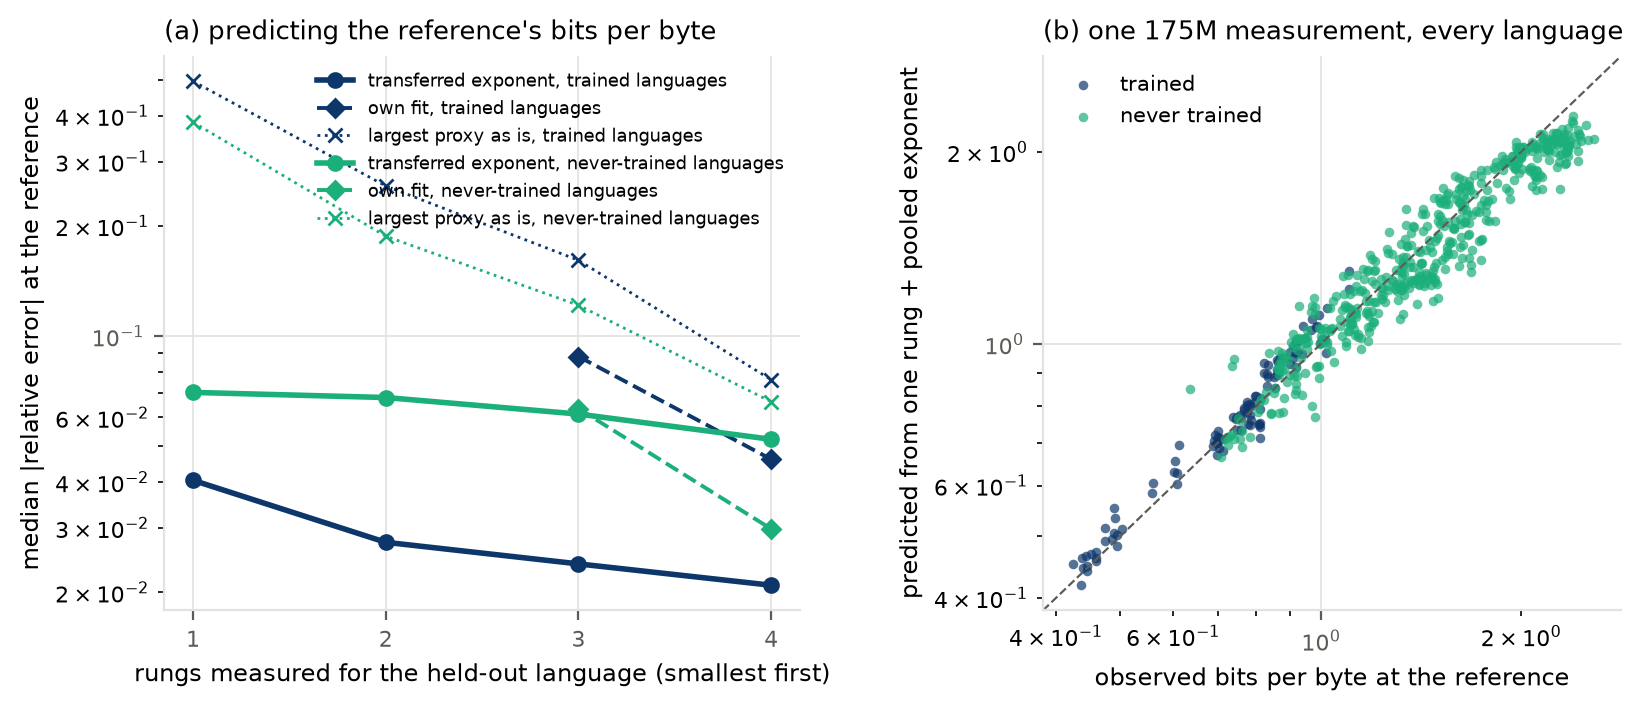
\includegraphics[width=\textwidth]{figures/rq5.png}
\caption{Transfer of scaling behaviour to held-out languages. (a) Median absolute relative error of the reference's bits per byte as a function of how many of the held-out language's smallest rungs are measured, with the exponent borrowed from the other languages (solid), fitted on the language itself (dashed, needs three rungs), or with no extrapolation at all (dotted), for languages present in or absent from the corresponding training mixture. (b) Predicted against observed reference bits per byte from a single 175M measurement per language.}
\label{fig:rq5}
\end{figure}

\textbf{Results.} Figure~\ref{fig:rq5} shows that pooling exponents across languages supports accurate extrapolation. The median exponent is 0.14 at $L = 1$, 0.16 to 0.17 at $L \in \{2, 8, 15, 30\}$ and 0.20 at $L = 50$, with a standard deviation across languages of 0.03 to 0.07. Consequently, the borrowed exponent with a single 175M measurement predicts the reference within a median 3.4\% for trained languages and 6.7\% for never-trained ones (Figure~\ref{fig:rq5}a), and 71\% of the never-trained predictions land within 10\%. For trained languages, adding measurements lowers the error to 2.1\% at three rungs, compared with 5.1\% for the language-specific fit. We hypothesize that pooling reduces sensitivity to noise in short scaling curves. The advantage is not uniform across training-exposure groups or numbers of measured rungs, Figure~\ref{fig:rq5}a also shows settings where the language-specific fit is competitive. The no-extrapolation baseline is 36 to 45\% off from one rung and still 6.5 to 7.3\% off from four. Never-trained languages are predicted with a small systematic bias (median signed error $-3.4$\%), under the convention $(\mathrm{predicted}-\mathrm{observed})/\mathrm{observed}$. The extrapolation therefore slightly underestimates their reference BPB and is optimistic about their performance. Panel (b) compares predictions with observations across a five-fold range of BPB; the identity line makes the direction of the residuals visible.

\textbf{Decision transfer.} Transferring a design ranking is less consistent than predicting BPB. On the languages neither scheme trains, the list decision is read correctly by 56\% at 175M, 68\% at 350M and 76\% at 600M and 1B, against 40, 100, 94 and 65\% on the trained languages. Agreement is higher on shared training languages at 350M and 600M, but this ordering reverses at 175M and 1B. Different proxy sizes also cover different language settings and references. These results support partial transfer of the language-list decision, rather than a general advantage for either language population. We leave the question of which language properties predict the residual to future work.
